\documentclass[12pt,aspectratio=1610]{beamer}
\RequirePackage{
    amsmath,
    amssymb,
    calc,
    cancel,
    booktabs,
    color,
    siunitx,
    tikz,
    wrapfig,
    array,
    leftidx,
    float,
    etoolbox,
    fancyhdr,
    longtable,
    hyperref,
    ltcaption,
    ulem,
    wasysym,
    accents,
    listings,
    tabularx,
}

\hypersetup{
    hidelinks,
    breaklinks              = true,
}

\usepackage[final]{pdfpages}
\usepackage[many]{tcolorbox}

\RenewDocumentCommand{\vec}{m}{\mathbf{#1}}

\makeatletter
    \def\new@mathgroup{\alloc@8\mathgroup\mathchardef\@cclvi}
    \patchcmd{\document@select@group}{\sixt@@n}{\@cclvi}{}{}
    \patchcmd{\select@group}{\sixt@@n}{\@cclvi}{}{}
\makeatother

\RequirePackage{mathspec}                                   % includes fontspec
\RequirePackage{polyglossia}                                % multi-language support
\RequirePackage{xunicode}
\setdefaultlanguage{slovak}

% Setup fonts -- see fontspec/mathspec documentation.
\defaultfontfeatures{
    Mapping         = tex-text,
    Scale           = MatchLowercase,
    Ligatures       = TeX
}


\NewDocumentCommand{\labelmath}{m +m}{%
    \begin{equation}%
        #2%
        \label{#1}%
    \end{equation}%
}

\NewDocumentCommand{\labelalign}{m +m}{%
    \begin{align}%
        #2%
        \label{#1}%
    \end{align}%
}

\linespread{1.0}
\setlength{\parindent}{0cm}
\setlength{\parskip}{6pt}
\setlength{\abovedisplayskip}{0mm}
\setlength{\belowdisplayskip}{0mm}
\setlength{\abovedisplayshortskip}{0mm}
\setlength{\belowdisplayshortskip}{0mm}
\setlength{\itemindent}{0pt}
\setlength{\textfloatsep}{0mm}
\setlength{\tabcolsep}{3mm}
\setlength{\LTcapwidth}{0.8\textwidth}
\renewcommand{\arraystretch}{1.2}

\setcounter{secnumdepth}{2}

/home/kvik/dgs/core/tex/math.tex
\DeclareSIUnit\au{AU}
\DeclareSIUnit\pixel{px}
\DeclareSIUnit\lightyear{ly}
\DeclareSIUnit\parsec{pc}
\DeclareSIUnit\earthmass{M_{\earth}}
\DeclareSIUnit\speedoflight{c}
\DeclareSIUnit\foe{foe}
\DeclareSIUnit\year{yr}
\DeclareSIUnit\eur{€}
\DeclareSIUnit\solarmass{M_{\astrosun}}
\DeclareSIUnit\solarluminosity{L_{\astrosun}}
\DeclareSIUnit{\byte}{B}




\linespread{1.0}
\setlength{\parindent}{0cm}
\setlength{\parskip}{6pt}
\setlength{\abovedisplayskip}{0mm}
\setlength{\belowdisplayskip}{0mm}
\setlength{\abovedisplayshortskip}{0mm}
\setlength{\belowdisplayshortskip}{0mm}
\setlength{\itemindent}{0pt}
\setlength{\textfloatsep}{0mm}
\setlength{\tabcolsep}{3mm}
\renewcommand{\arraystretch}{1.2}

\setcounter{secnumdepth}{0}

\NewDocumentCommand{\fspicture}{m O{W} O{black}}{
    {
        \setbeamertemplate{navigation symbols}{}
        \setbeamercolor{background canvas}{bg = #3}
        \begin{frame}[plain]
            \begin{tikzpicture}[remember picture, overlay]
                \node[at=(current page.center)] {
                    \ifstrequal{H}{#2}{                                  
                        \includegraphics[height=\paperheight]{#1}%
                    }{%
                        \includegraphics[width=\paperwidth]{#1}%
                    }
                };
            \end{tikzpicture}
        \end{frame}
    }
}

\NewDocumentCommand{\frejm}{m +m}{
    \begin{frame}
        \frametitle{#1}
        #2
    \end{frame}
}

\NewDocumentCommand{\fragfrejm}{m +m}{
    \begin{frame}[fragile]
        \frametitle{#1}
        #2
    \end{frame}
}

\defbeamertemplate{description item}{align center}{\hfill\insertdescriptionitem\hfill}
\definecolor{desc}{rgb}{0.66, 0, 0}
\definecolor{citem}{rgb}{0.72, 0, 0}
\definecolor{csitem}{rgb}{0.90, 0, 0}
\definecolor{cssitem}{rgb}{1, 0.1, 0.1}
\definecolor{qprimarybg}{rgb}{0.95, 0.95, 0.95}
\definecolor{check}{rgb}{0, 0.8, 0}
\definecolor{coded}{rgb}{0.9, 0.9, 0.9}
\definecolor{todo}{rgb}{1.0, 0.3, 0.3}
\definecolor{model}{rgb}{0.75, 0, 0}

\setbeamertemplate{navigation symbols}{}
\newfontfamily{\semibold}{Segoe UI Semibold}
\RenewDocumentCommand{\emph}{m}{{\semibold#1}}
\NewDocumentCommand{\code}{m}{\textcolor{desc}{\texttt{#1}}}
\NewDocumentCommand{\model}{m}{\colorbox{coded}{\textcolor{model}{\texttt{#1}}}}
\NewDocumentCommand{\todo}{m}{\colorbox{todo}{#1}}

\mode<presentation> {
    \usetheme{Szeged}
    \usecolortheme{beaver}
    
    \usefonttheme{professionalfonts}
    \setallmainfonts{Minion Pro}
    \setmathrm{Minion Pro}
    
    \setsansfont{Segoe UI}
    \setmonofont{Consolas}
    \setbeamercolor*{enumerate item}{fg = citem}
    \setbeamercolor*{enumerate subitem}{fg = csitem}
    \setbeamercolor*{enumerate subsubitem}{fg = cssitem}
    \setbeamercolor*{description item}{fg = desc}
    \setbeamercolor*{itemize item}{fg = citem}
    \setbeamercolor*{itemize subitem}{fg = csitem}
    \setbeamercolor*{itemize subsubitem}{fg = cssitem}
    \setbeamercolor*{palette primary}{fg = red, bg = qprimarybg}
}

\newcommand<>\highlightbox[2]{%
    \alt#3{\makebox[\dimexpr\width-2\fboxsep]{\colorbox{#1}{#2}}}{#2}%
}

\AtBeginSection[]{
    \subsection{\insertsection}
    \begin{frame}
        \vfill
        \centering
        \begin{beamercolorbox}[sep = 18pt, center, shadow = true, rounded = true]{title}
            \usebeamerfont{title}\insertsectionhead%
            \vfill
        \end{beamercolorbox}
        \vfill
    \end{frame}
}

\makeatletter
% Render percent sign with nice font, not ugly Computer modern
    \mathcode`\%="7025

% Fixes mathspec bug -- URL numbers are rendered with wrong font
    \ernewcommand\eu@MathPunctuation@symfont{Latin:m:n}
    \DeclareMathSymbol{,}{\mathpunct}{\eu@MathPunctuation@symfont}{`,}
    \DeclareMathSymbol{?}{\mathpunct}{\eu@MathPunctuation@symfont}{`?}
    \DeclareMathSymbol{.}{\mathord}{\eu@MathPunctuation@symfont}{`.}
    \DeclareMathSymbol{<}{\mathrel}{\eu@MathPunctuation@symfont}{`<}
    \DeclareMathSymbol{>}{\mathrel}{\eu@MathPunctuation@symfont}{`>}
    \DeclareMathSymbol{/}{\mathord}{\eu@MathPunctuation@symfont}{`/}
    \DeclareMathSymbol{;}{\mathpunct}{\eu@MathPunctuation@symfont}{`;}
    \DeclareMathSymbol{(}{\mathopen}{\eu@DigitsArabic@symfont}{`(}
    \DeclareMathSymbol{)}{\mathclose}{\eu@DigitsArabic@symfont}{`)}
    \XeTeXDeclareMathSymbol{^^^^2026}{\mathinner}{\eu@MathPunctuation@symfont}{"2026}[\mathellipsis]
    \DeclareMathSymbol{0}{\mathalpha}{\eu@DigitsArabic@symfont}{`0}
    \DeclareMathSymbol{1}{\mathalpha}{\eu@DigitsArabic@symfont}{`1}
    \DeclareMathSymbol{2}{\mathalpha}{\eu@DigitsArabic@symfont}{`2}
    \DeclareMathSymbol{3}{\mathalpha}{\eu@DigitsArabic@symfont}{`3}
    \DeclareMathSymbol{4}{\mathalpha}{\eu@DigitsArabic@symfont}{`4}
    \DeclareMathSymbol{5}{\mathalpha}{\eu@DigitsArabic@symfont}{`5}
    \DeclareMathSymbol{6}{\mathalpha}{\eu@DigitsArabic@symfont}{`6}
    \DeclareMathSymbol{7}{\mathalpha}{\eu@DigitsArabic@symfont}{`7}
    \DeclareMathSymbol{8}{\mathalpha}{\eu@DigitsArabic@symfont}{`8}
    \DeclareMathSymbol{9}{\mathalpha}{\eu@DigitsArabic@symfont}{`9}
\makeatother


\title{Meteor(oid?) models and density estimation}
\subtitle{}
\author{\small \emph{Martin Baláž}}
\institute{DAA colloquium}
\date{2020--02--26}

\begin{document}
    {
        \usebackgroundtemplate{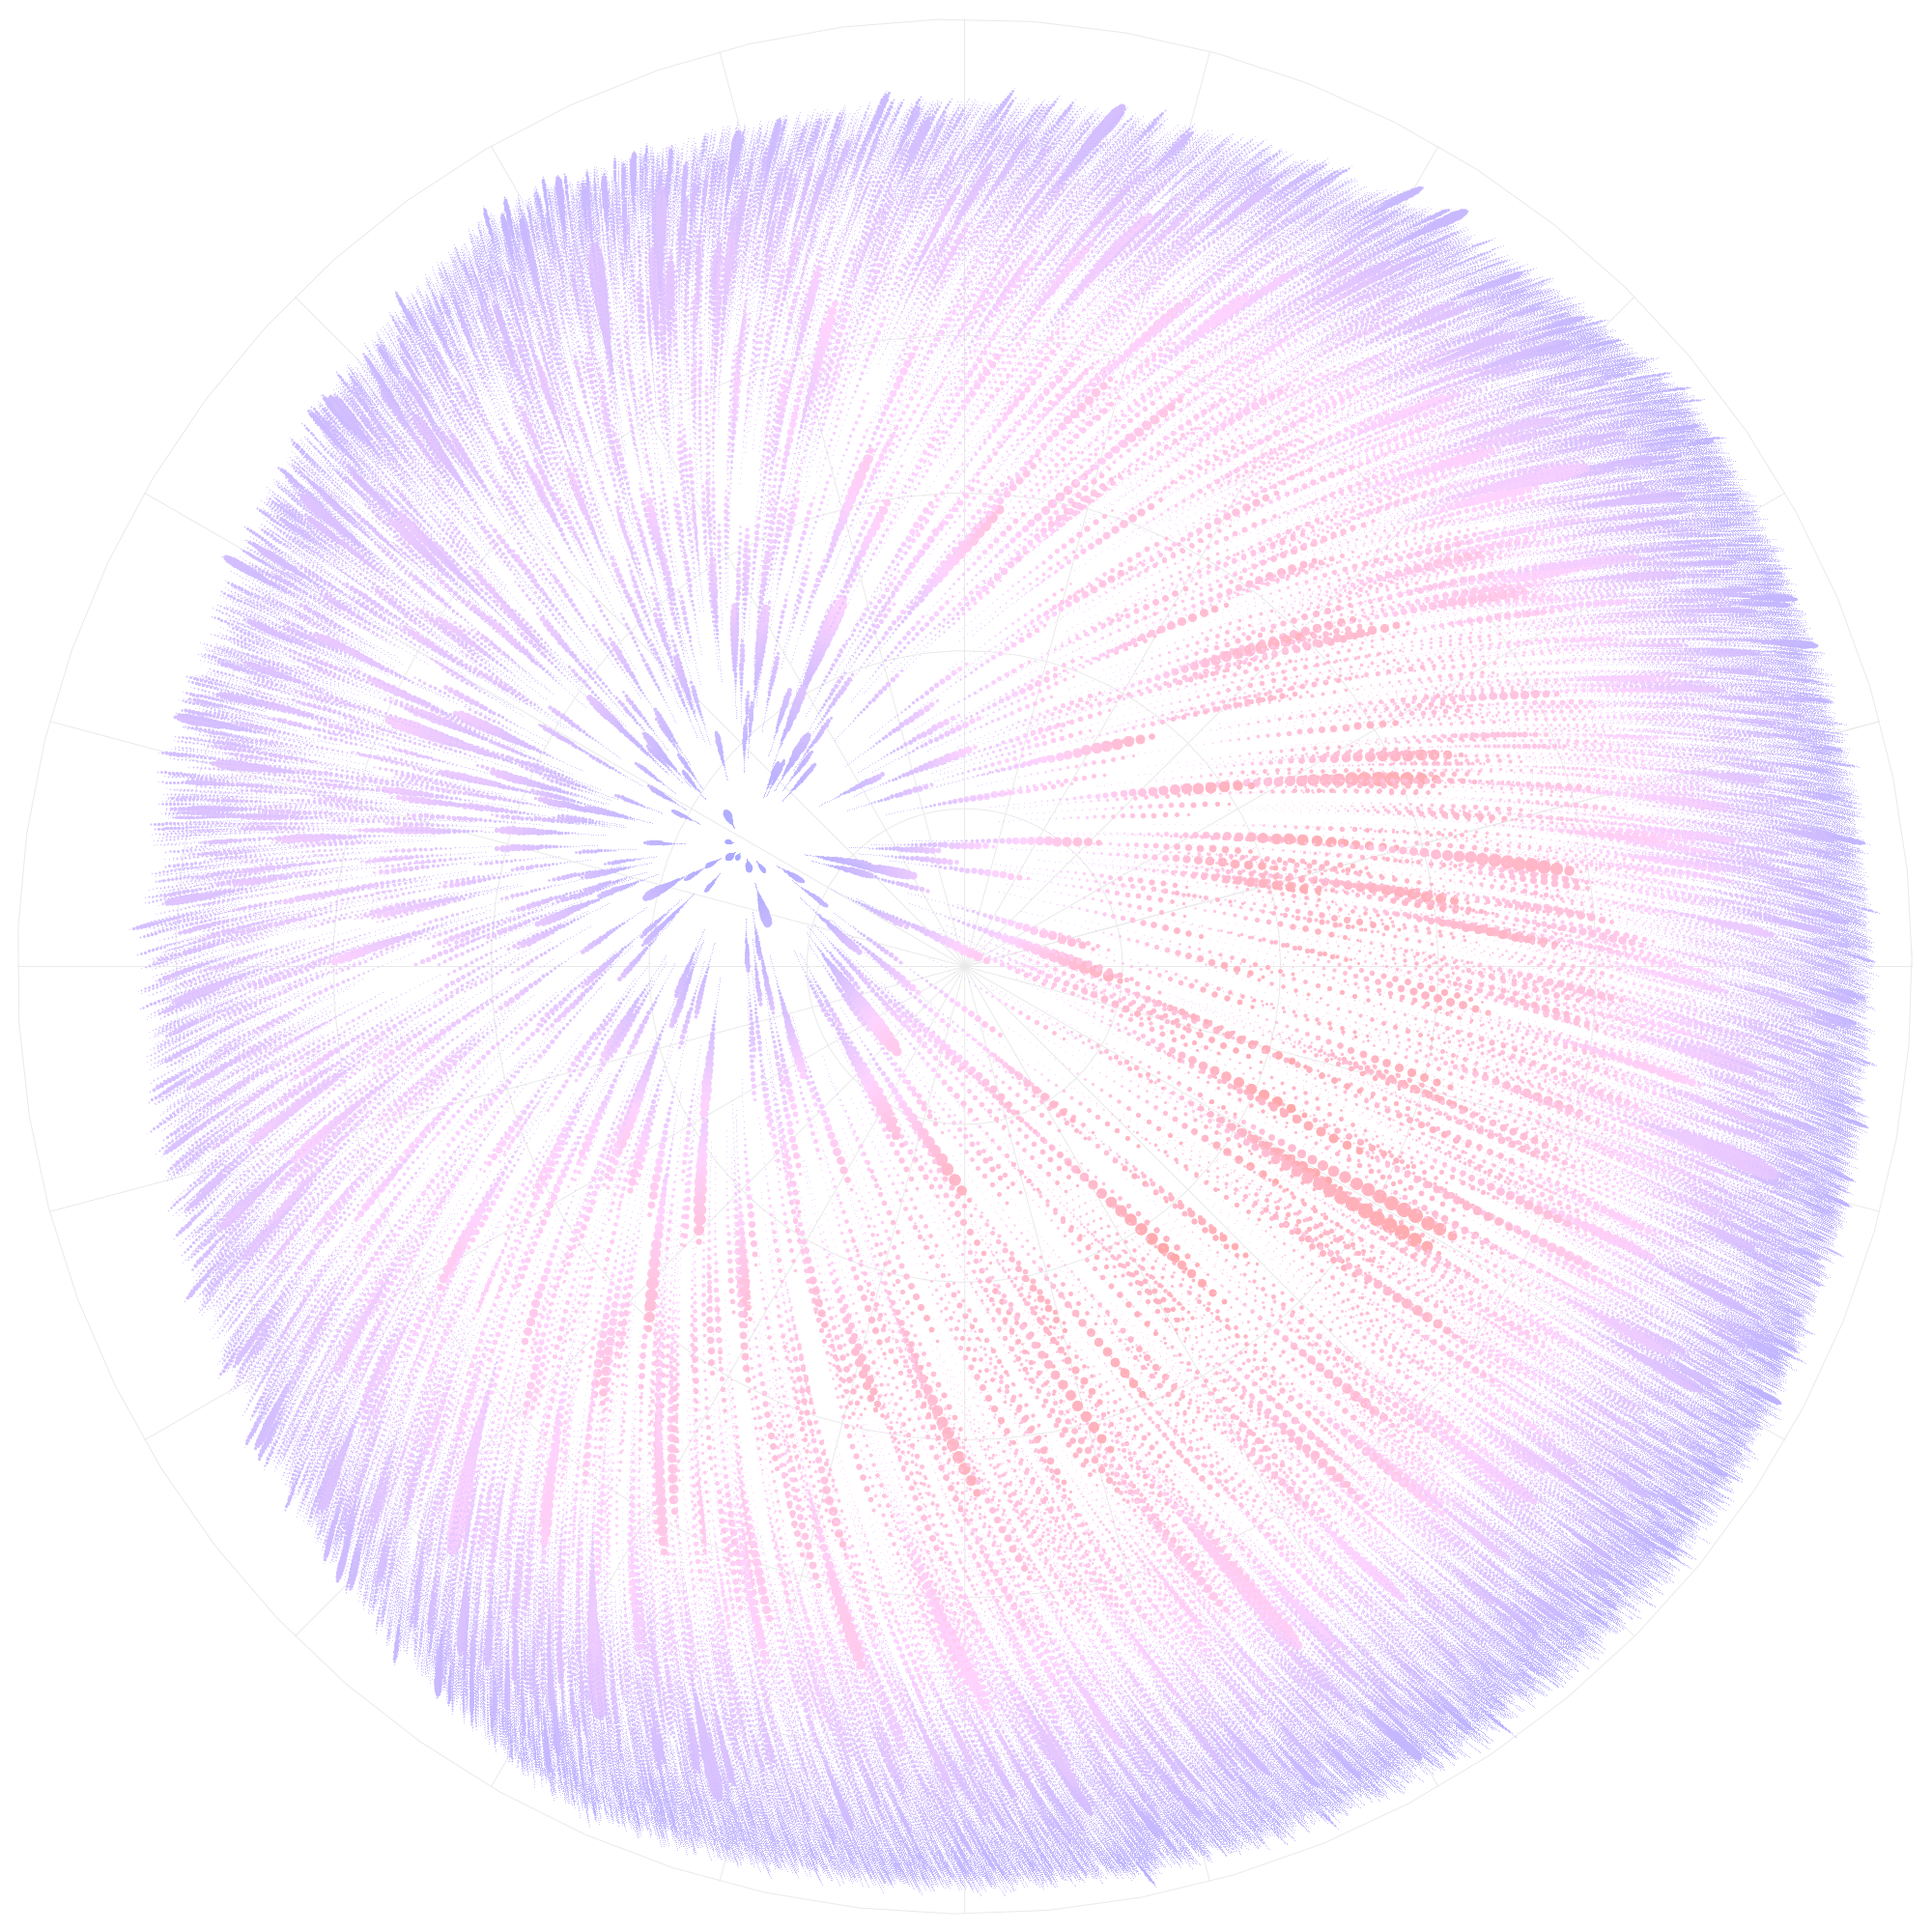
\includegraphics[width=\paperwidth]{pictures/fireworks-i.png}}
        \begin{frame}
            \titlepage
        \end{frame}
    }
    \section{Overview}
        \frejm{Motivation}{
            We want to develop a model of meteors and meteoroids
            \pause
            \begin{itemize}
                \item density
                \item flux
                \item activity in time
                \item magnitudes
                \item $r$ or $s$ index
                \item ...
            \end{itemize}
        }

        \frejm{Model}{
            Build a map / prediction
            \begin{itemize}
                \item we have
                \begin{itemize}
                    \item observations by AMOS
                    \item model of meteoroid entry
                    \item simulation toolkit ASMODEUS
                \end{itemize}
                \pause
                \item we want
                \begin{itemize}
                    \item describe meteor \emph{distribution}
                    \item devise a suitable \emph{model}
                \end{itemize}
            \end{itemize}
        }

    \setbeamersize{description width = 5mm}

    \section{Parametric estimation}
        \frejm{Introduction}{
            Sometimes we know what to expect...
            \begin{itemize}
                \item assume normal distribution
                \item establish the values of $\sigma$ and $\mu$
            \end{itemize}
        }

        \frejm{Algorithm}{
            \begin{itemize}
                \item define the class of distributions
                \item try some parameters
                \item minimize the \emph{error metric}
                \begin{itemize}
                    \item gradient descent
                    \item simulated annealing
                    \item ...
                \end{itemize}
            \end{itemize}
        }

        \frejm{Case study I: heights of people}{
        }

       % \fspicture{gauss-1.png}

        \frejm{Case study II: height by sex}{
            We can extract information from the distribution
            \begin{itemize}
                \item assume males and females, both normally distributed
            \end{itemize}
            $$
                F(x; c_\text{\male}, \mu_\text{\male}, \sigma_\text{\male}, c_\text{\female}, \mu_\text{\female}, \sigma_\text{\female}) =
                \frac{c_\text{\male}}{\sqrt{2\pi}\sigma_\text{\male}} e^{\frac{-\left(x - \mu_\text{\male}\right)^2}{2\sigma_\text{\male}^2}} +
                \frac{c_\text{\female}}{\sqrt{2\pi}\sigma_\text{\female}} e^{\frac{-\left(x - \mu_\text{\female}\right)^2}{2\sigma_\text{\female}^2}}
            $$
            \pause
            \begin{itemize}
                \item we need to find values of all parameters
            \end{itemize}
        }

        \frejm{Summary}{
            \begin{itemize}
                \item advantages
                \begin{itemize}
                    \item simple
                    \item can extract information
                \end{itemize}
                \item disadvantages
                \begin{itemize}
                    \item we have to know the distribution
                    \item dependent on binning
                    \begin{itemize}
                        \item both \emph{scale} and \emph{shift}
                    \end{itemize}
                    \item there must be many data points
                \end{itemize}
            \end{itemize}
        }

    \section{Non-parametric methods}
        \frejm{No parameters}{
            Sometimes this all is not applicable...
            \pause
            \begin{itemize}
                \item the distribution is not \emph{known} beforehand
                \pause
                \item there are \emph{too many} parameters or minima
                \pause
                \item no suitable metric
            \end{itemize}
        }

        \frejm{Histograms}{
            We may group samples together
            \begin{itemize}
                \item well known discrete method
                \pause
                \item sometimes \emph{normalized}
            \end{itemize}
        }

        \frejm{Bin width}{
            \begin{itemize}
                \item usually we set bin width manually
                \begin{itemize}
                    \item rounding
                    \item shifting
                \end{itemize}
                \pause
                \item there are ±rigorous methods of determination of optimal bin width
            \end{itemize}
            $$
                w = 2 \cdot \mathrm{IQR} \cdot N^{-1/3}
            $$
        }

        \frejm{Shifting}{
            Bin position is also important
            \centering
            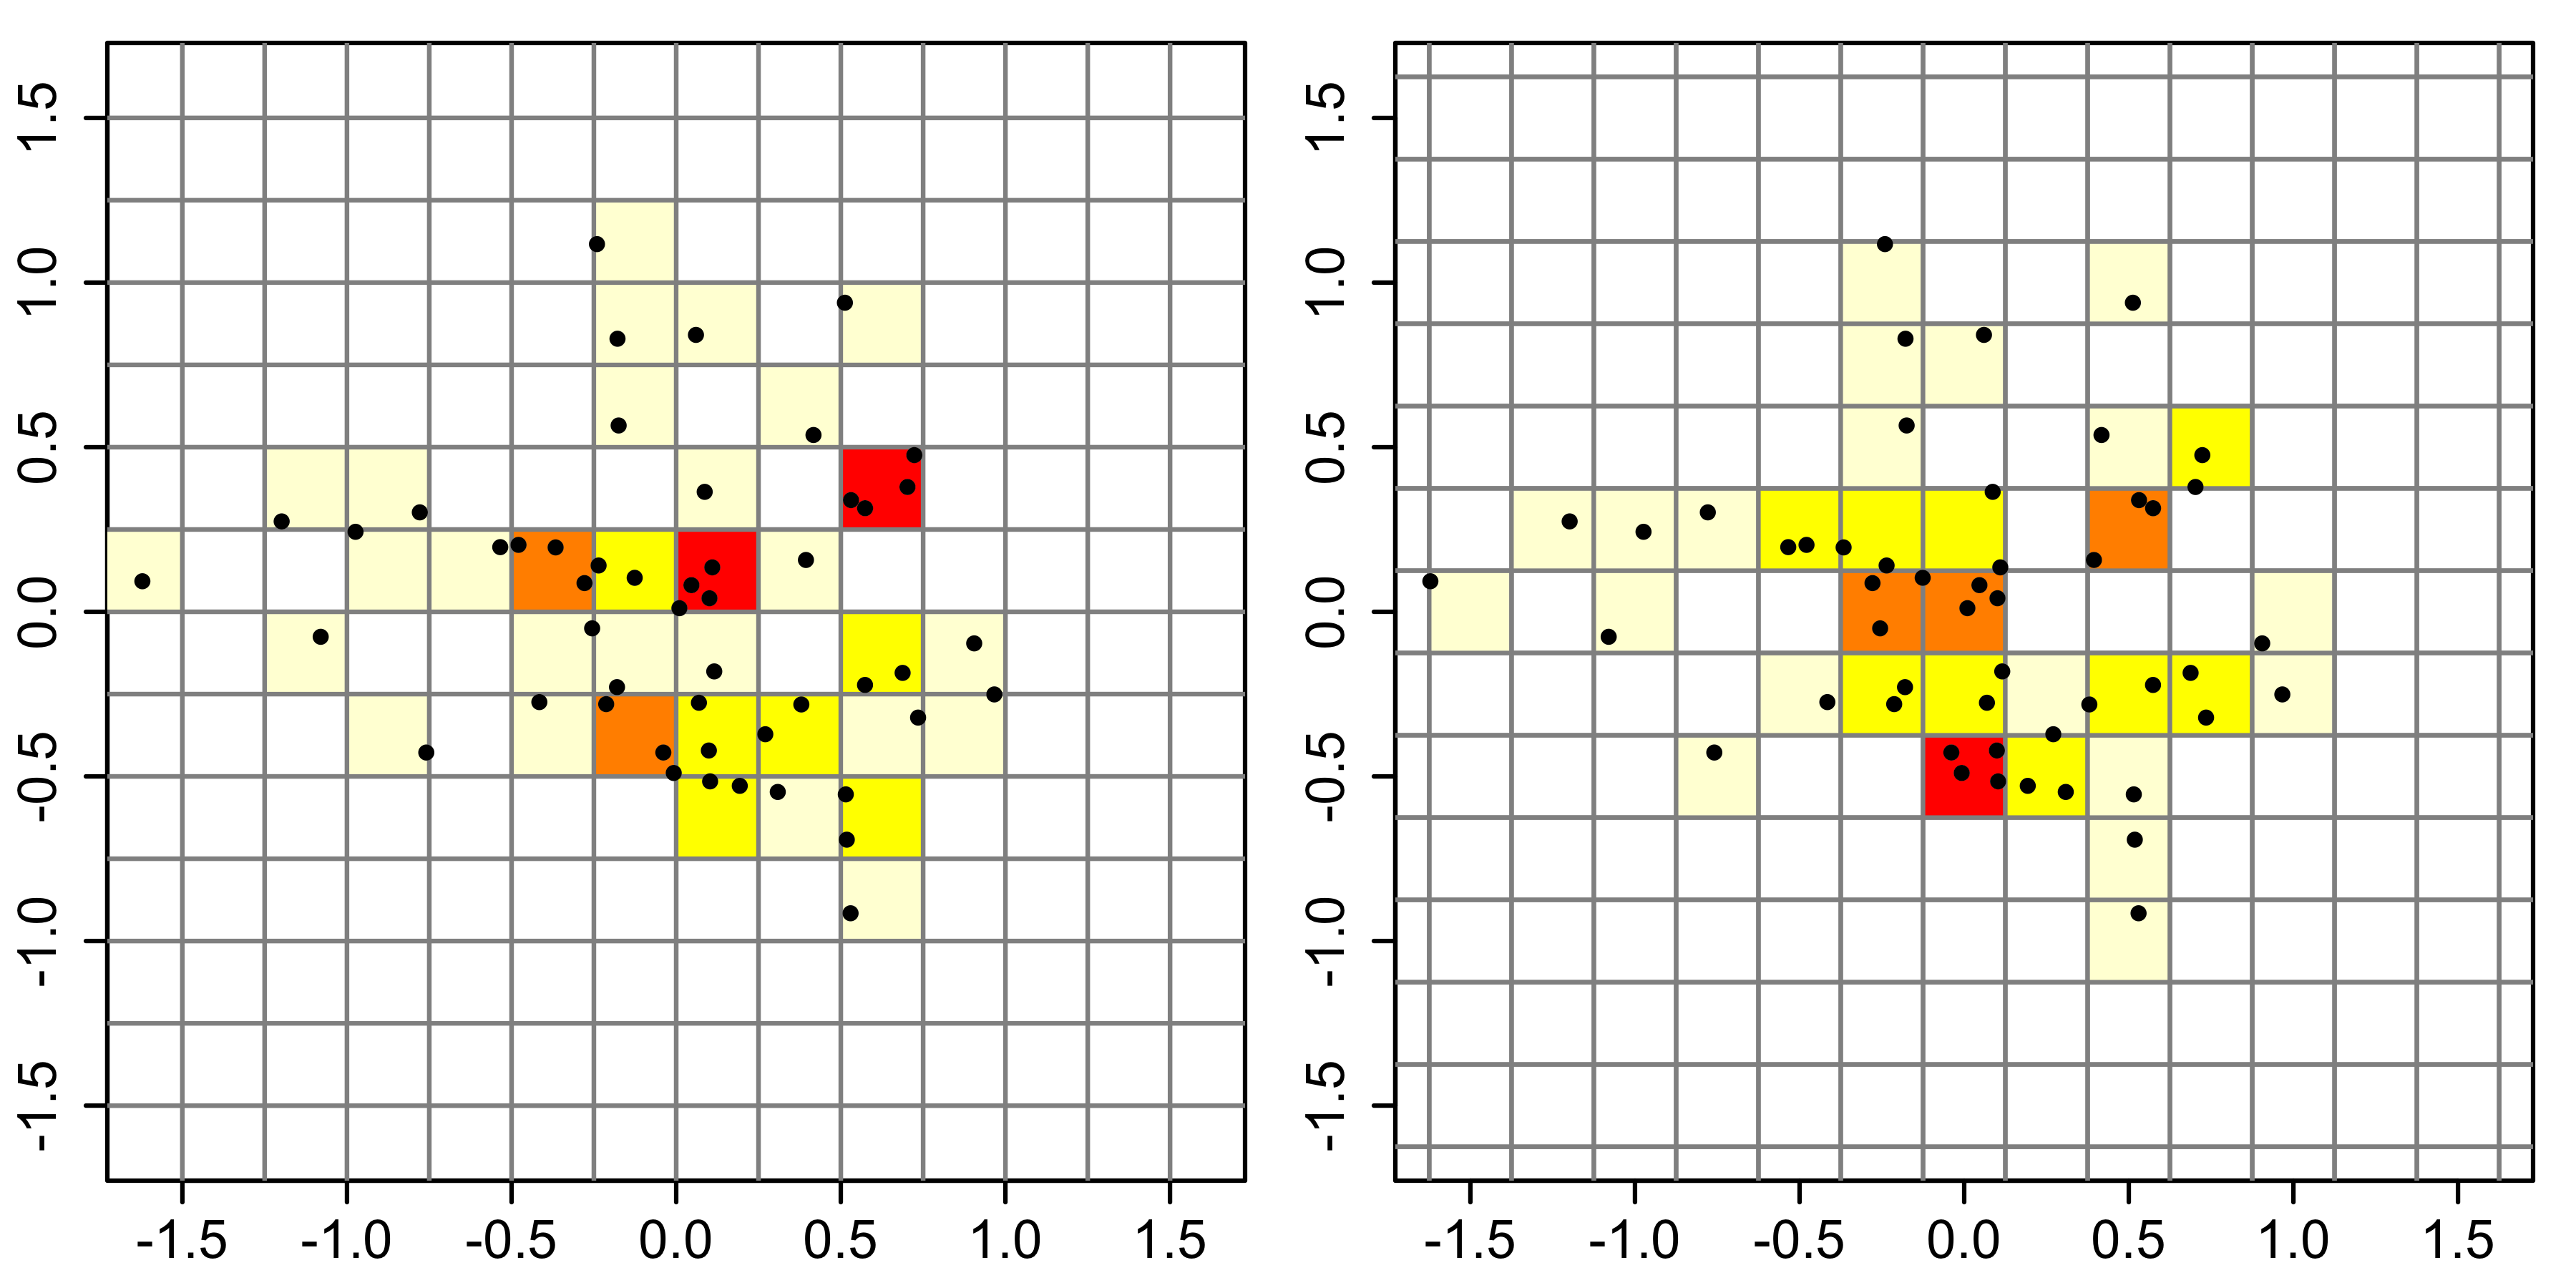
\includegraphics[width = 0.9\linewidth]{pictures/shift.png}
        }


    \section{Kernel density estimation}
        \frejm{One dimension}{
            We can generalize histograms to continuous case
            \begin{itemize}
                \item camera vs human eye
                \item paper?
            \end{itemize}
        }

        \frejm{Bandwidth}{
            \begin{itemize}
                \item similar to bin width in histograms
            \end{itemize}
            $$
                \Hat[-1pt]{f}(\vec{x}) = \frac{1}{nh} \Sum[i = 1][n]{K\left(h \left(x - x_i\right)\right)}
            $$
        }

        \frejm{Goodness of fit}{
            If we know the true distribution, we can design a metric
            \begin{itemize}
                \item \emph{MISE}
            \end{itemize}
            $$
                \mathrm{MISE}(\Hat[-1pt]{f}(x), f\,(x)) = \Int[\mathbb{R}]{\left(\Hat[-1pt]{f}(x) - f\,(x) \right)^2}{x}
            $$

            \begin{itemize}
                \item samples still \textbf{can} originate in a weird distribution
            \end{itemize}
        }

        \frejm{Multiple dimensions}{
            KDE easily \emph{generalizes} to multivariate functions
            \begin{itemize}
                \item but the variables may be \emph{correlated}
            \end{itemize}
        }

        \frejm{Example}{
            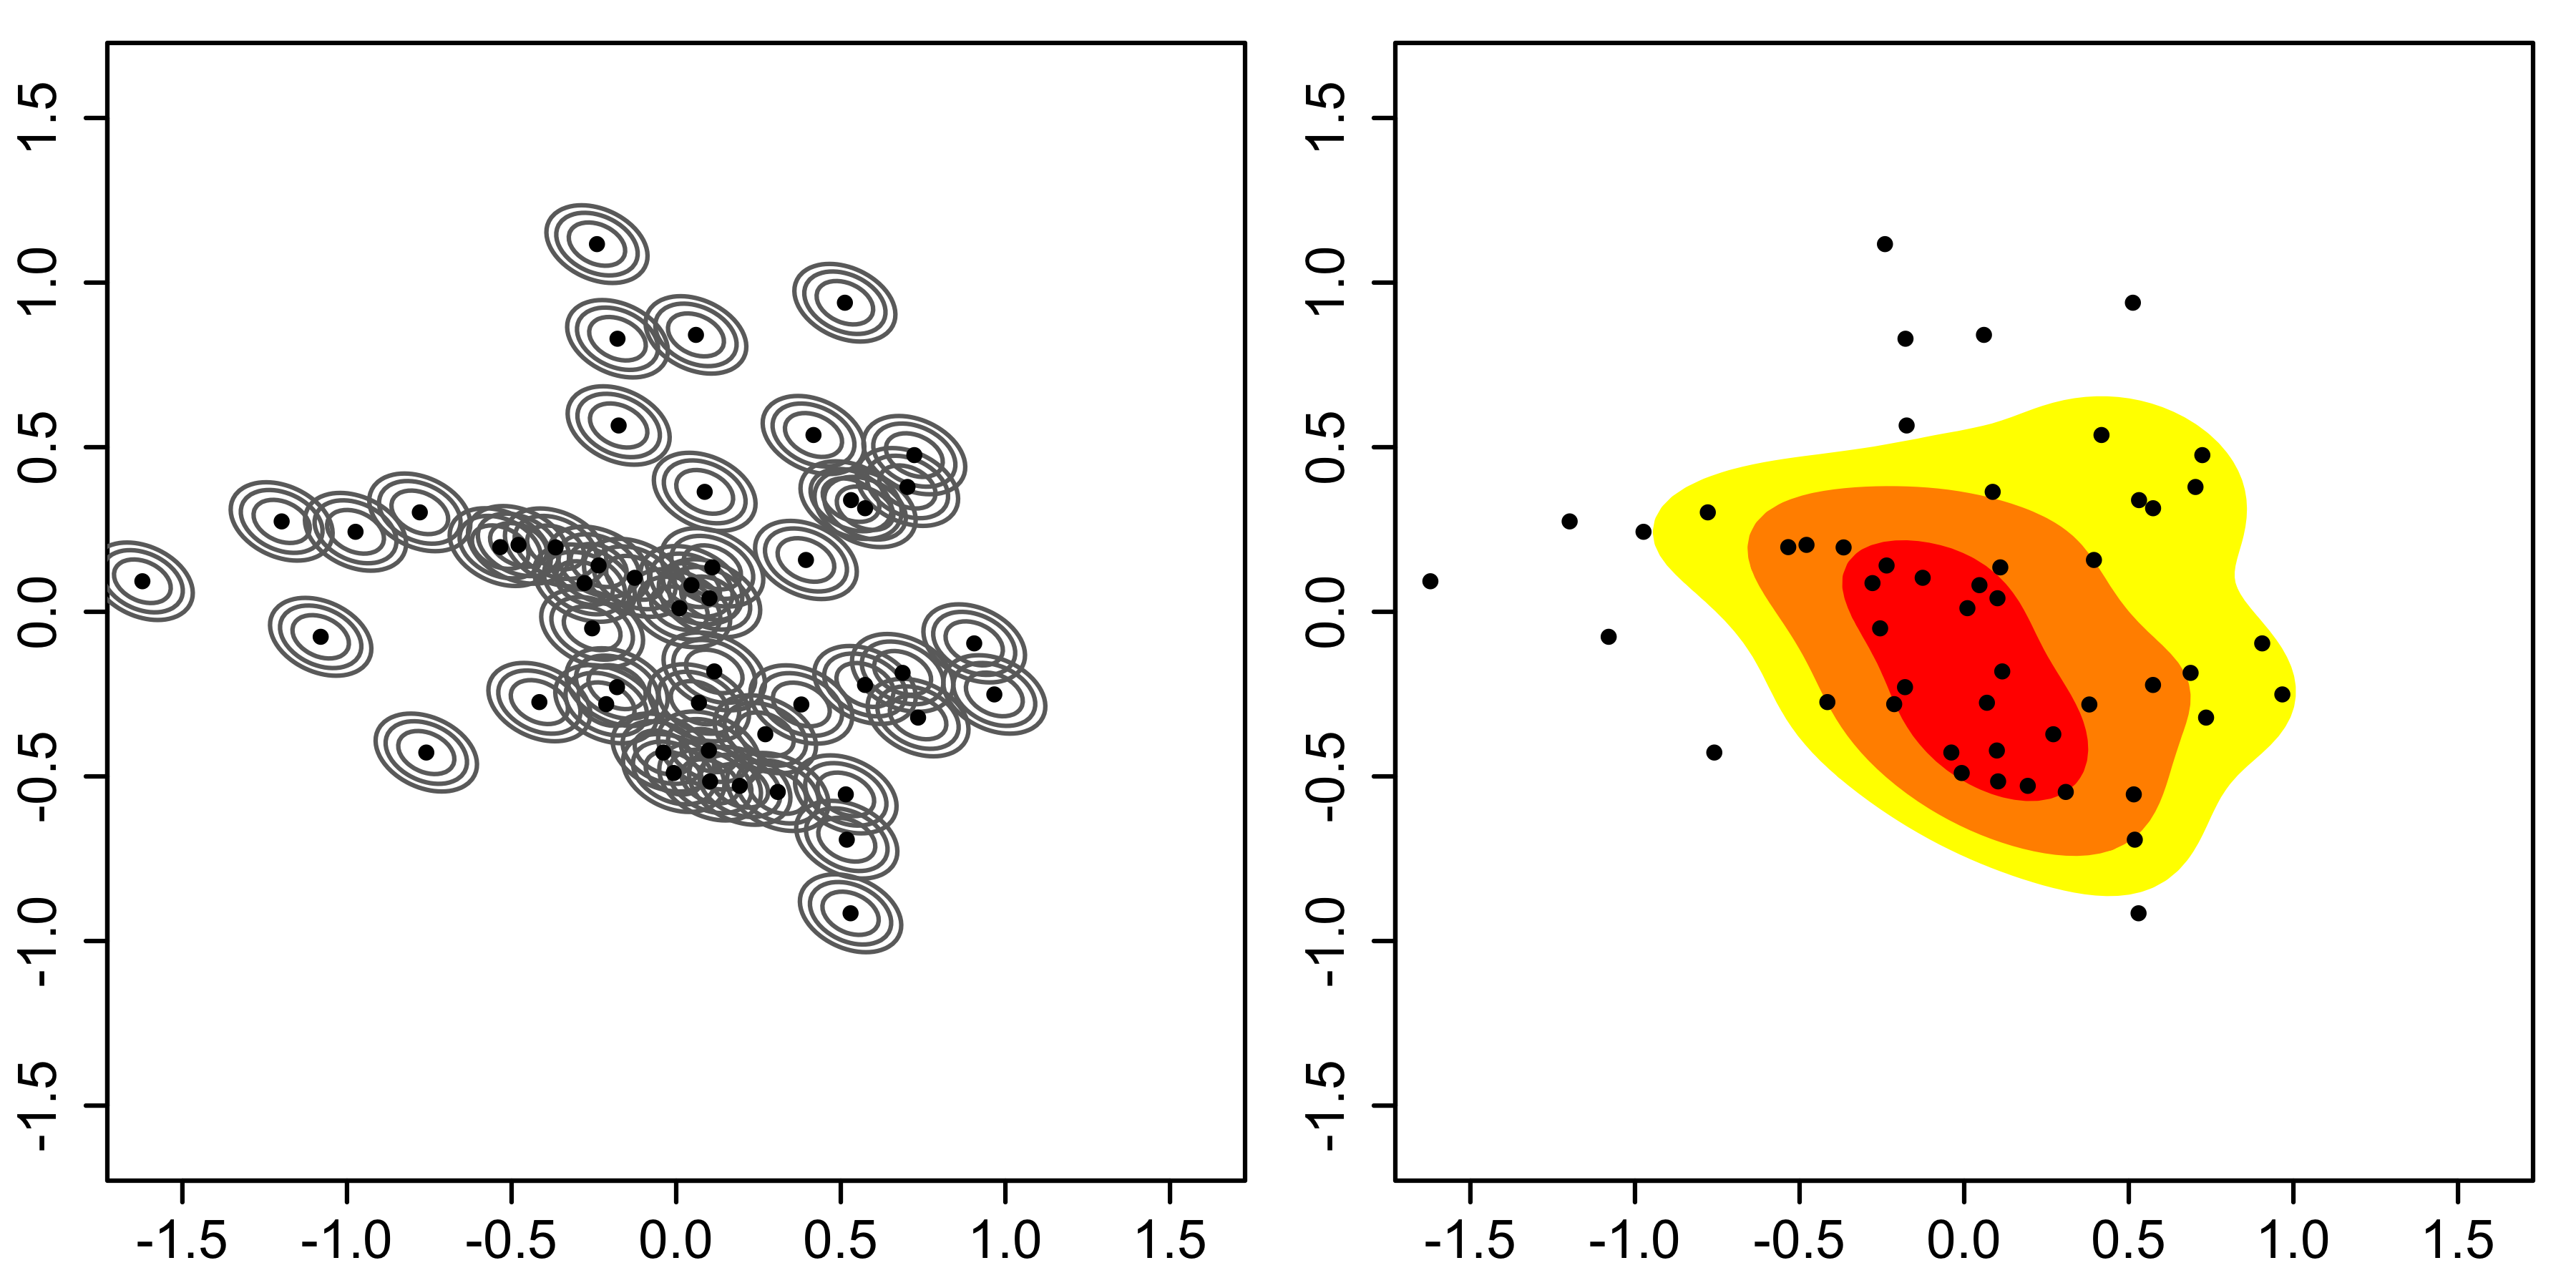
\includegraphics[width = \linewidth]{pictures/kde.png}
        }

        \frejm{Correlation}{
            $$
                \Hat[-1pt]{f}(\vec{x}) = \frac{1}{n \Abs{\vec{H}}} \Sum[i = 1][n]{K\left(\vec{H}^{-1}\left(\vec{x} - \vec{x}_i\right)\right)}
            $$
        }

        \frejm{Convolution}{
            KDE can be defined as a convolution
            \begin{itemize}
                \item mathematically beautiful
                \item but not very practical
            \end{itemize}
        }

        \frejm{Adaptive KDE}{
            Bandwidth need not be constant
            \begin{itemize}
                \item sometimes it is beneficial to vary $h$
                \pause
                \item generally
                \begin{itemize}
                    \item narrow bandwidth where data are \emph{abundant}
                    \item wide bandwidth where data are \emph{sparse}
                \end{itemize}
            \end{itemize}
        }

    \section{Models}
        \frejm{What is this good for?}{
            \begin{itemize}
                \item we want to find PDFs for \emph{meteors} and \emph{meteoroids}
                \pause
            \item devise \emph{two models}
            \end{itemize}
        }

        \frejm{Observational model}{
            We may estimate the distribution of meteors in the sky
            \begin{itemize}
                \item<1-> time (1)
                \item\only<2>{positions}\only<3->{\sout{positions}}
                \item<3-> radiants (3 or 2+1)
                \item<4-> magnitude spectrum (1)
            \end{itemize}
            $$
                \only<5->{
                    \mathcal{A}(t, \vec{v}, m) \equiv \mathcal{A}(t, \delta_\mathrm{R}, \alpha_\mathrm{R}, v_\infty, m).
                }
            $$
        }

        \fspicture{pictures/model.png}[][white]

        \frejm{Orbital model}{
            Observational model tells \emph{when} and \emph{what}...
            \pause
            but does not tell \emph{why}
            \pause
            \begin{itemize}
                \item time (1)
                \pause
                \item position (3)
                \pause
                \item velocity (3)
                \pause
                \item mass spectrum (1)
            \end{itemize}
            \pause
            $$
                \mathcal{M}_{\mathrm{rv}}(t, \vec{r}, \vec{v}, \mu) \quad\text{or}\quad
                \mathcal{M}_{\mathrm{oe}}(t, a, e, i, \omega, \Omega, T, \mu)
            $$
            \pause
            or better
            $$
                \mathcal{M}_{\mathrm{rv}}(t, \vec{r}, \vec{v}, \log \mu) \quad\text{or}\quad
                \mathcal{M}_{\mathrm{oe}}(t, 1/a, e, i, \omega, \Omega, T, \log \mu)
            $$
        }

        \frejm{Curse of dimensionality}{
            $N$-volume of parameter space increases exponentially
            \begin{itemize}
                \item the space is \emph{vast}
                \pause
                \item $\ang{360} \times \ang{180} \times \num{8766} \times \num{50} \times \num{50} \approx \num{1.42e12}$
                \pause
                \item almost all of it is ``in the corner''
                \item distance metrics are not very useful
            \end{itemize}
        }


    \section{Summary}
        \frejm{References}{
            \begin{itemize}
                \item \textbf{Hwang, J.-N. -- Lay, S.-R. and Lippman, A.}:
                    Nonparametric multivariate density estimation: a case study.
                    IEEE Transactions on Signal Processing 42, 1994.
                \item \textbf{Vida, D. -- Brown, P. -- Campbell-Brown, M.}:
                    Modeling the measurement accuracy of pre-atmosphere velocities of meteoroids. MNRAS 479, 2018
                \item \textbf{Vida, D. -- Brown, P. -- Campbell-Brown, M.}:
                    Generating realistic synthetic meteoroid orbits. Icarus 296, 2017.
            \end{itemize}
        }
\end{document}
